
\documentclass{article}
\usepackage{fullpage}

\usepackage[T1]{fontenc}
\usepackage[utf8]{inputenc} 
\usepackage{lmodern}
\usepackage[slovene]{babel}

\usepackage{graphicx}


\makeindex

\linespread{1.1}

\title{Dynamic Time Warping \\ (Dinamično časovno krivljenje)}
\author{Maja Abraham, Tine Fabiani}
\date{\today}

\begin{document}
    
\maketitle

\section{Naloga}
Predstavi razdaljo Dynamic Time Warping (DTW) in jo implementiraj na 
realnih podatkih. Poskušaj jo uporabiti kot razdaljo za grupiranje podatkov (clustering), za
iskanje nekakšne mediane,... 
\section{Opis DTW razdalje}
Dynamic Time Warping je algoritem, ki se uporablja za merjenje podobnosti dveh
časovnih zaporedji, ki pa se lahko razlikujeta v hitrosti. \\
DTW nam pove kako dobro se dve časovni zapordji ujemata,
pri tem pa moramo upoštevati naslednja pravila:
\begin{itemize}
    \item Vsak indeks iz prvega zaporedja se mora ujemati z enim ali več indeksi iz drugega zaporedja in obratno.
    \item Prvi indeks iz prvega zaporedja se mora ujemati s prvim indeksom iz drugega zaporedja (vendar ni nujno, da je to njegovo edino ujemanje).
    \item Zadnji indeks iz prvega zaporedja se mora ujemati z zadnjim indeksom iz drugega zaporedja (vendar ni nujno, da je to njegovo edino ujemanje).
    \item Preslikava indeksov iz prvega zaporedja v indekse iz drugega zaporedja mora biti monotono naraščajoča in obratno.
    
\end{itemize}

\underline{\textsc{Optimalno ujemanje}} je ujemanje, ki zadostuje vsem omejitvam in pravilom, pri čemer je vsota absolutnih razlik za vsak ujemajoči
 se par indeksov med njihovimi vrednostmi minimalen.

 % slika : https://www.researchgate.net/publication/350397933/figure/fig2/AS:1005448887025665@1616729103138/Simple-visualization-of-dynamic-time-warping-DTW-alignment-Instead-of-assuming-a.jpg
\begin{figure}[h!]
    \centering
    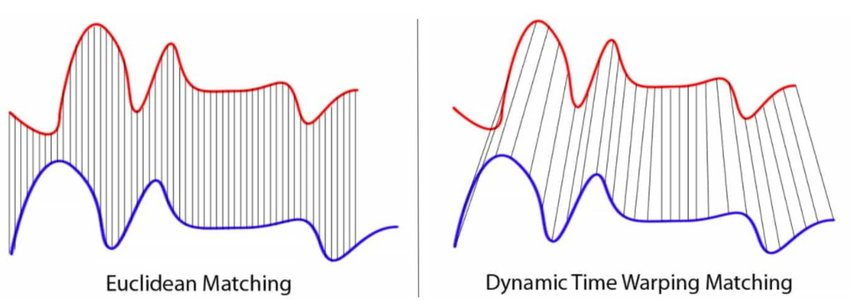
\includegraphics[scale=0.37]{dtw1.png}
    \caption{Vizualna predstava rezultatov DTW}
\end{figure}

 \section{Upraba DTW}
Algoritem se pogosto uprablja za:
\begin{itemize}
    \item  za obdelavo avdio podatkov. V avdio sistemih se uporablja za prpozavnje zvokov govora, ki lahko imajo različno hitrost govorenja.  
    \item pogosta uporaba v financah je ocenjevanje kvalitete napovednih modelov v primerjavi z resničnimi podatki. 
\end{itemize}

% slika: https://www.databricks.com/wp-content/uploads/2019/04/dynamic-time-warping.png

\begin{figure}[h!]
    \centering
    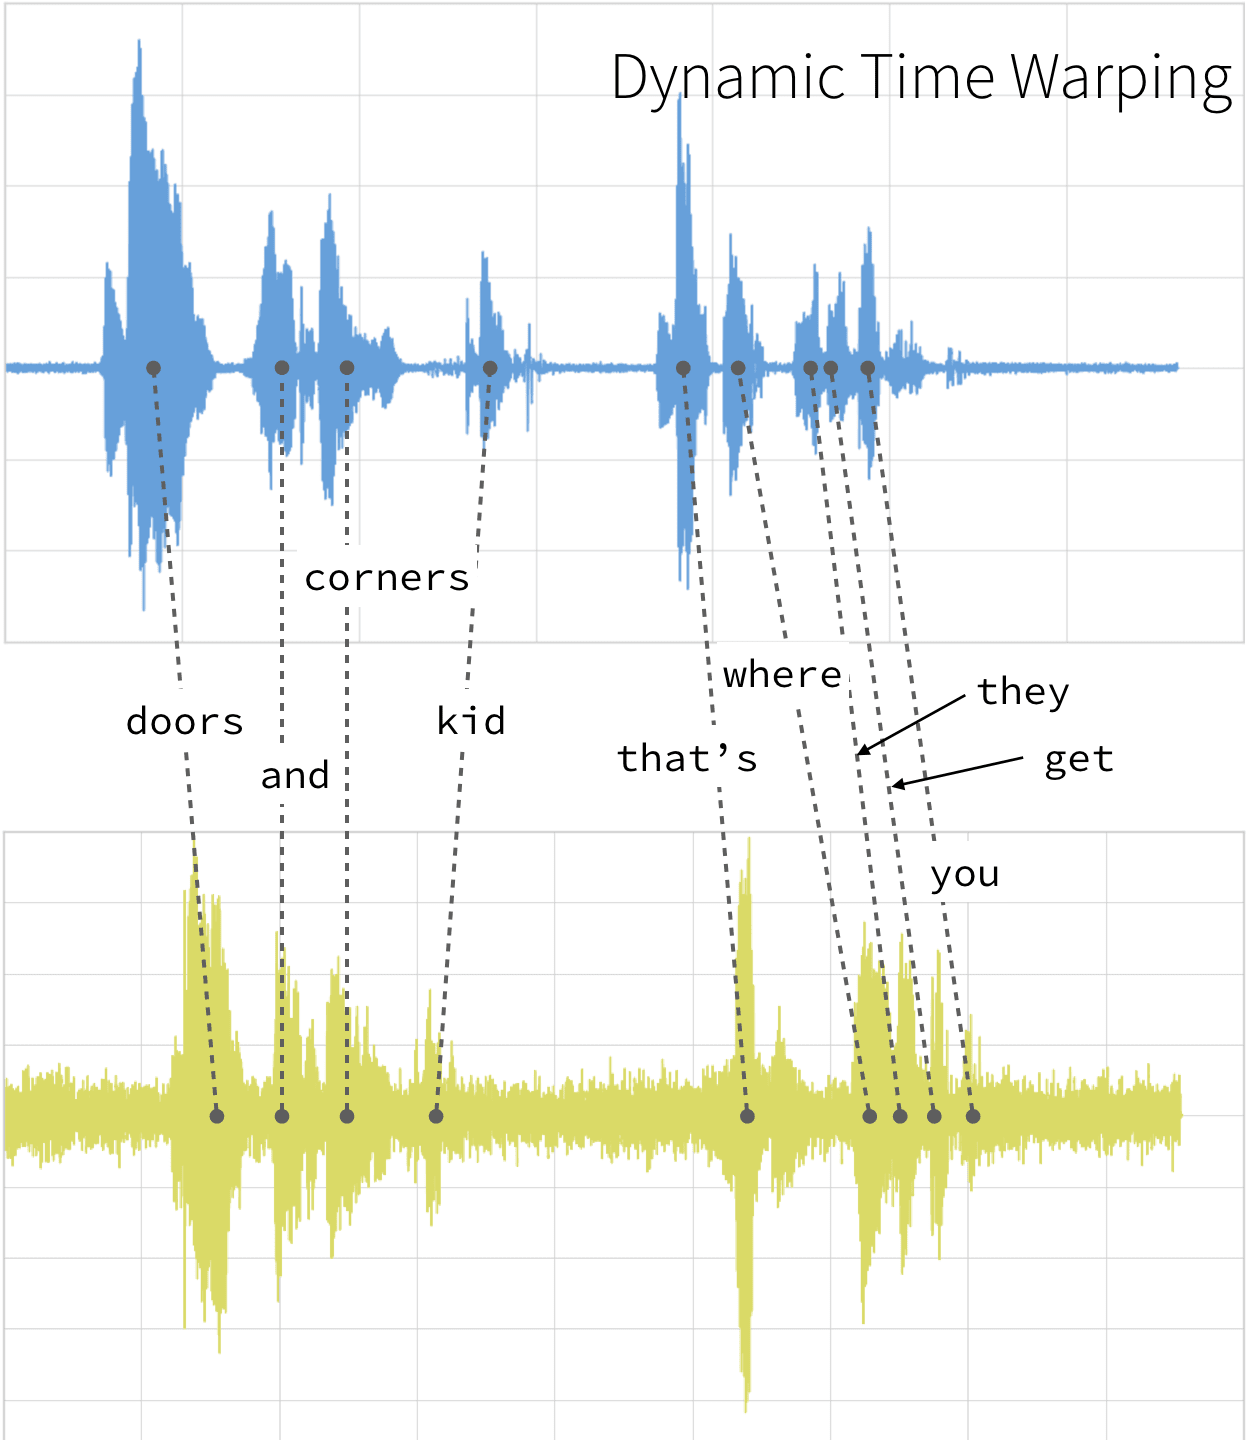
\includegraphics[scale=0.15]{dynamic-time-warping.png}
    \caption{Uporaba DTW na zvočnih podatkih}
\end{figure}


\section{Načrt dela}
V nalogi bova najprej podrobneje predstavila algoritem DTW in njegovo implementacijo s pomočjo dinamičnega programiranja. 
Opazila sva povezavo z konceptom iskanja najkrajše razdalje med nizi, ki ga bova uporabila za implementacijo. 
Zapisala bi algortem DTW v izbranem programskem okolju. Na kratko bi predstavila primere uprabe DTW algoritma. 
Algoritem bi dopolnila z grupiranjem podatkov. Uporabljala bova programsko okolje \textbf{Python} ali \textbf{R}, 
ki vsebuje paket \textbf{dtw} za delo z DTW algoritmom.
Za zaključek bi na konkretnih podatkih uporabila sam algoritem in analizirala rezultate. 
\end{document}